% ════════════════════════════════════════════════════════════════════
% Chapter 4 — Synchronisation Strategy
% ════════════════════════════════════════════════════════════════════
\section{Hardware-Level Synchronisation Strategy}\label{sec:sync}

Temporal synchronisation is the most critical engineering challenge in multimodal kinematic data collection.
A synchronisation error of just \SI{10}{\milli\second} between the IMU and camera streams---less than one camera frame period---introduces a velocity error proportional to the barbell's jerk (rate of change of acceleration).
During the ``sticking point'' of a heavy squat, where acceleration can change by \SI{5}{\metre\per\second\squared} in \SI{10}{\milli\second}, a \SI{10}{\milli\second} timing misalignment produces a systematic velocity bias of \SI{0.05}{\metre\per\second}---equal to the entire width of a velocity training zone.

Software-based synchronisation approaches (NTP, PTP, or host-side timestamp matching) are fundamentally inadequate for this application.
They suffer from unpredictable OS scheduling delays (typically \SI{1}{}--\SI{15}{\milli\second} on Linux), USB bus arbitration jitter, and thermal drift between independent crystal oscillators.
Our system therefore implements a \emph{direct hardware synchronisation topology} that eliminates all software-timing dependencies.


\subsection{The D455 Master Pulse}

The D455 camera is configured as the system timing master (\code{hw\_sync\_mode = 1}).
At the precise start of exposure for every depth frame, the camera drives a physical \texttt{FRAME\_SYNC} pulse on Pin~5 of its 9-pin auxiliary connector.
At \SI{90}{fps}, this pulse fires exactly every \SI{11.111}{\milli\second} with sub-microsecond jitter (governed by the D455's internal PLL).

This output signal is a \SI{1.8}{\volt} CMOS logic level.


\subsection{The NPN Level-Shifting Circuit}\label{sec:level_shifter}

The ESP32 and the ICM-42688-P both operate at \SI{3.3}{\volt} logic levels.
The ESP32's nominal input-high voltage threshold is $V_{IH} \approx 0.75 \times V_{DD} = \SI{2.475}{\volt}$, which exceeds the \SI{1.8}{\volt} camera output.
While empirical testing showed that the physical silicon threshold often sits lower (around \SI{1.4}{}--\SI{1.6}{\volt}), relying on out-of-spec behaviour is unacceptable for a research platform that must produce reliable data across temperature variations and unit-to-unit silicon variability.

We therefore designed and built a discrete NPN transistor level-shifting circuit.
Two circuit topologies were evaluated, and the recommended Option~A (non-inverting, two-transistor) was implemented.
The complete schematic and bill of materials are shown in \cref{fig:level_shifter}.

\begin{figure}[H]
  \centering
  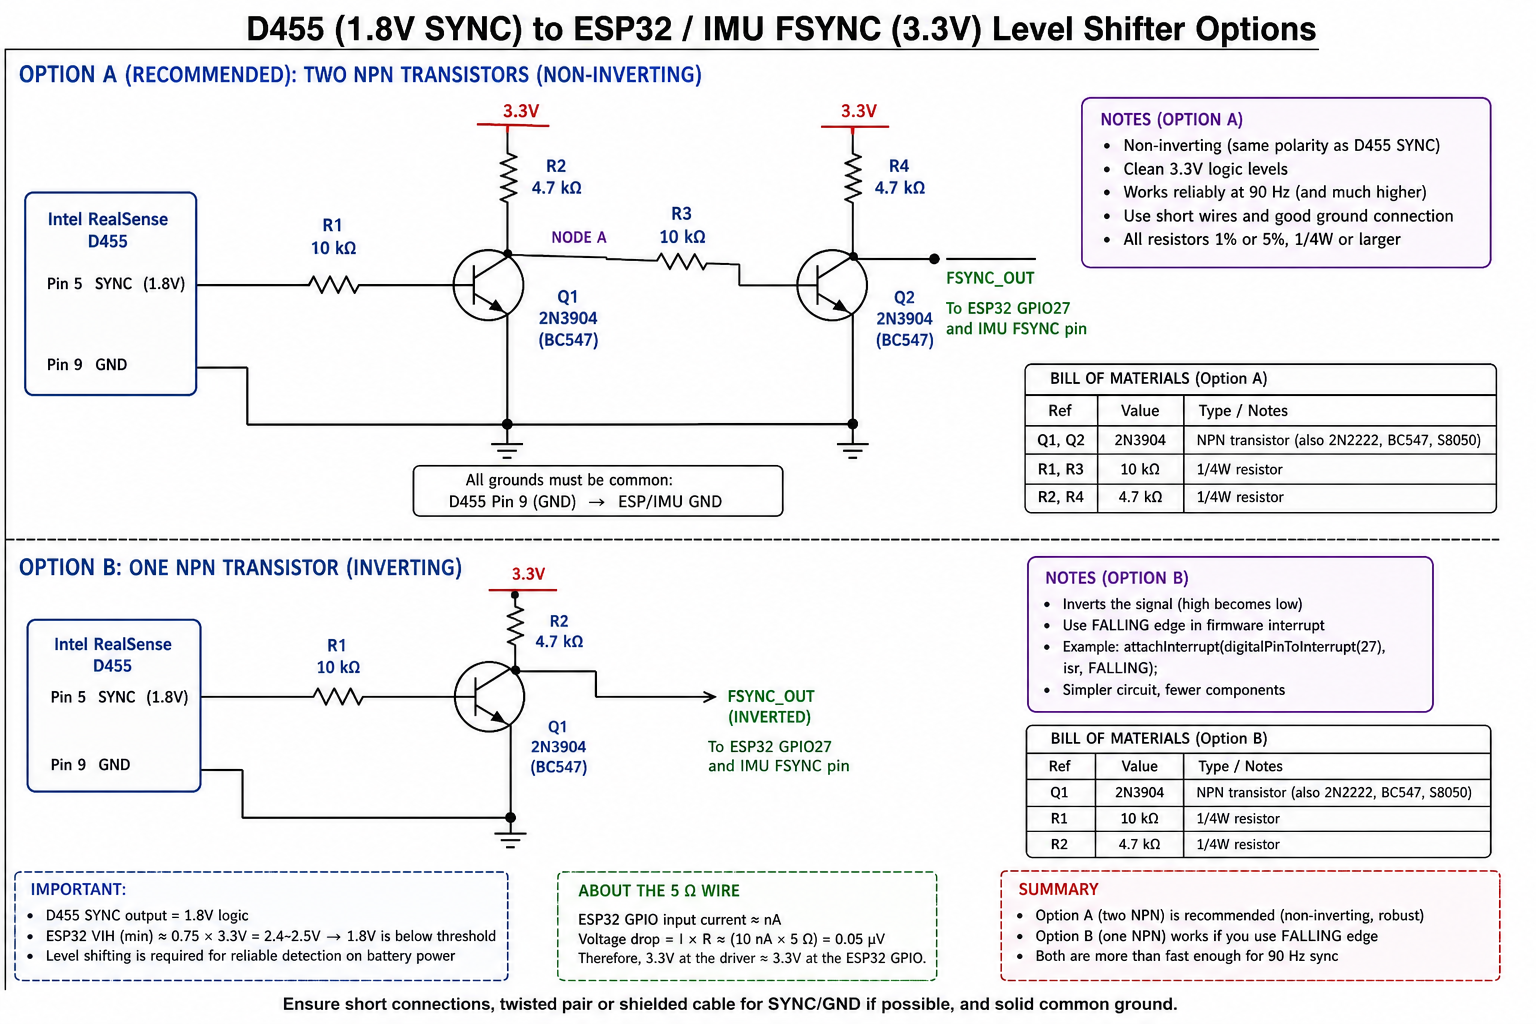
\includegraphics[width=\textwidth]{fig_level_shifter.png}
  \caption{Complete level-shifter schematic showing both evaluated topologies. Option~A (top, recommended) uses two 2N3904 NPN transistors in a non-inverting configuration, preserving the SYNC polarity. Option~B (bottom) uses a single transistor but inverts the signal, requiring a \code{FALLING}-edge interrupt configuration in firmware.}
  \label{fig:level_shifter}
\end{figure}

\subsubsection{Option A: Non-Inverting Two-Transistor Circuit (Implemented)}

The recommended circuit uses two 2N3904 (or equivalent BC547/S8050) NPN transistors:
\begin{itemize}[nosep]
  \item \textbf{Q1 (First Stage):} The D455 SYNC output (Pin~5, \SI{1.8}{\volt}) drives the base of Q1 through a \SI{10}{\kilo\ohm} current-limiting resistor (R1). Q1's collector is pulled up to \SI{3.3}{\volt} via a \SI{4.7}{\kilo\ohm} resistor (R2). When SYNC goes HIGH, Q1 turns on, pulling NODE~A LOW. This constitutes the first inversion.
  \item \textbf{Q2 (Second Stage):} NODE~A drives the base of Q2 through a \SI{10}{\kilo\ohm} resistor (R3). Q2's collector is pulled up to \SI{3.3}{\volt} via a \SI{4.7}{\kilo\ohm} resistor (R4). When NODE~A goes LOW (Q1 on), Q2 turns off, and the output (\code{FSYNC\_OUT}) is pulled HIGH to \SI{3.3}{\volt}. This constitutes the second inversion, restoring the original polarity.
\end{itemize}

The result is a clean \SI{3.3}{\volt} output that faithfully reproduces the input polarity with a propagation delay $<\SI{100}{\nano\second}$---negligible relative to the \SI{11.1}{\milli\second} frame period.

\subsubsection{Bill of Materials}

\begin{table}[H]
  \centering
  \caption{Bill of Materials for the level-shifting circuit (Option A).}
  \label{tab:bom}
  \begin{tabular}{llll}
    \toprule
    \textbf{Ref} & \textbf{Value} & \textbf{Type} & \textbf{Notes} \\
    \midrule
    Q1, Q2   & 2N3904  & NPN transistor          & Also BC547, 2N2222, S8050 \\
    R1, R3   & \SI{10}{\kilo\ohm}  & $\nicefrac{1}{4}$\,W resistor & 1\% or 5\% tolerance \\
    R2, R4   & \SI{4.7}{\kilo\ohm} & $\nicefrac{1}{4}$\,W resistor & 1\% or 5\% tolerance \\
    \bottomrule
  \end{tabular}
\end{table}

\subsubsection{Grounding}
All ground planes must be common: D455 Aux Pin~9 (GND) $\rightarrow$ ESP32 GND $\rightarrow$ ICM-42688-P GND.
Short connections, twisted-pair or shielded cable for the SYNC/GND pair, and solid common grounding are essential for reliable edge detection at \SI{90}{\hertz}.


\subsection{FSYNC Signal Routing}

The level-shifted \SI{3.3}{\volt} \code{FSYNC\_OUT} signal is routed simultaneously to two destinations:
\begin{enumerate}[nosep]
  \item \textbf{ESP32 GPIO\,27:} Configured as a rising-edge interrupt input.
  \item \textbf{ICM-42688-P Pin~9 (FSYNC):} Configured via Bank~1 register \reg{INTF\_CONFIG5} (\code{0x7B}) to accept the FSYNC function (value \code{0x02}, setting bits[2:1] = 01).
\end{enumerate}

Both chips therefore receive the identical physical edge at the same instant, guaranteeing zero inter-chip synchronisation skew.


\subsection{IMU FSYNC Tagging Engine}\label{sec:fsync_tagging}

When the \SI{3.3}{\volt} edge arrives at the ICM-42688-P FSYNC pin, the IMU's internal tagging engine records the event directly into the sensor data payload.
The tagging is configured via \reg{FSYNC\_CONFIG} (address \code{0x62}):

\begin{itemize}[nosep]
  \item \textbf{Bits [6:4] = 001:} Selects the Least Significant Bit of \reg{TEMP\_DATA0} as the tag target. When a FSYNC event is detected, this bit is forced to~1 in the next data-ready sample.
  \item \textbf{Bit [1] = 1} (\code{FSYNC\_UI\_FLAG\_CLEAR\_SEL}): The tag remains latched until the host performs a SPI read of the tagged register. This is critical because the camera runs at \SI{90}{\hertz} while the IMU is sampled at \SI{1}{\kilo\hertz}; without latching, the transient tag would be overwritten by the next internal UI register update before the ESP32 has a chance to read it.
  \item \textbf{Bit [0] = 0} (\code{FSYNC\_POLARITY}): Configures the FSYNC engine to trigger on the rising edge, matching the non-inverting level-shifter output polarity.
\end{itemize}

The complete register write is: \code{writeReg(0x62, 0x12)}.

Additionally, the internal timestamp counter is enabled via \reg{TMST\_CONFIG} (\code{0x54}) with value \code{0x1B}, enabling:
\begin{itemize}[nosep]
  \item \code{TMST\_TO\_REGS\_EN}: Latch the 16-bit internal timestamp counter at the FSYNC edge.
  \item \code{TMST\_RESOL = 1}: \SI{1}{\micro\second} timestamp resolution.
  \item \code{TMST\_FSYNC\_EN}: Enable FSYNC-triggered timestamp capture.
  \item \code{TMST\_EN}: Enable the timestamp counter.
\end{itemize}

The captured 16-bit timestamp can be read from \reg{TMST\_FSYNCH/L} (address \code{0x2B--0x2C}), providing the IMU-clock time of the FSYNC edge with \SI{1}{\micro\second} resolution.


\subsection{ESP32 Interrupt Handler and Debouncing}

On the ESP32 side, GPIO\,27 is configured with an interrupt on the \code{RISING} edge.
Even with the level-shifted signal, the rising edge may exhibit brief ringing as the transistor switches, potentially causing multiple spurious ISR firings within a few microseconds.
Since genuine camera frames are separated by $\geq$\SI{10}{\milli\second}, a strict temporal debounce window of \SI{5}{\milli\second} is implemented directly in the ISR:

\begin{lstlisting}[language=C++, caption={Camera trigger ISR with debounce logic.}, label={lst:isr_debounce}]
static void IRAM_ATTR isr_cam_trigger() {
    int64_t now = esp_timer_get_time();
    if ((now - g_last_cam_trig_us) < 5000) return;  // 5 ms debounce
    g_cam_trig_count++;
    g_last_cam_trig_us = now;
}
\end{lstlisting}

This handler provides two independent pieces of synchronisation information:
\begin{enumerate}[nosep]
  \item The \textbf{count} of camera trigger events (\code{g\_cam\_trig\_count}), which should match the FSYNC hit count from the IMU's temperature LSB tagging.
  \item The \textbf{ESP32 timestamp} of each trigger event (\code{g\_last\_cam\_trig\_us}), which can be correlated with the camera's hardware timestamp for the corresponding frame.
\end{enumerate}

The 5-second status report periodically prints both the camera trigger rate and the FSYNC hit count, allowing the operator to verify in real-time that both chips are detecting the same edges.


\subsection{Host-Side Temporal Alignment: The SyncEngine}\label{sec:sync_engine}

On the host PC, the \class{SyncEngine} class maintains a unified timeline by building a live affine mapping between the three independent clock domains:
\begin{enumerate}[nosep]
  \item \textbf{ESP32 clock:} 64-bit microsecond counter (\code{esp\_timer\_get\_time()}).
  \item \textbf{D455 hardware clock:} Reported as Unix-epoch seconds via the \code{RS2\_FRAME\_METADATA\_SENSOR\_TIMESTAMP} field with \code{GLOBAL\_TIME} domain.
  \item \textbf{Host monotonic clock:} \code{std::chrono::steady\_clock}, used as the common reference.
\end{enumerate}

\subsubsection{FSYNC-Based Hardware Anchor Pairs}
Every IMU sample whose temperature LSB is set (\code{fsync\_tagged = true}) was captured at the exact same physical instant as a camera frame trigger.
The \class{SyncEngine} registers these events from both streams:
\begin{lstlisting}[language=C++, numbers=none]
void register_imu_fsync_event(uint64_t esp_us, double host_s);
void register_camera_frame(double cam_hw_s, double host_s);
\end{lstlisting}
Pairing is performed by nearest-neighbour matching on the host timestamp.
From the accumulated pairs $(t_{\text{esp},i},\; t_{\text{cam},i})$, the engine fits a linear model:
\begin{equation}\label{eq:affine_sync}
  t_\text{cam} = a \cdot t_\text{esp} + b
\end{equation}
where $a \approx 10^{-6}$ (seconds per microsecond, i.e., unity scaling) and $b$ captures the fixed offset.
This affine fit is refreshed continuously as new pairs arrive, with a sliding window of up to 256 pairs, making the system self-calibrating and robust to slow thermal drift.

\subsubsection{Tap-Test Calibration}
Before each session, a mandatory ``tap test'' is performed.
The operator sharply taps the IMU sensor against a rigid surface near the camera.
This produces a massive, instantaneous acceleration spike ($>\SI{2}{\g}$) in the IMU data stream and a simultaneous visual displacement in the camera depth frame.
The \class{SyncEngine} cross-correlates the two signals to extract:
\begin{itemize}[nosep]
  \item \textbf{Temporal offset} ($\mu$s): the systematic delay between the two clock domains.
  \item \textbf{Clock drift} (ppm): the rate of divergence between the ESP32 crystal and the D455 ASIC clock.
  \item \textbf{Correlation quality} (0--1): confidence in the computed alignment.
\end{itemize}

\subsubsection{Drift Monitoring and Auto-Rearm}
During recording, the \class{SyncEngine} continuously monitors clock drift.
If drift exceeds \SI{100}{ppm} for a sustained period of \SI{5}{\second}, the \code{rearm\_required()} flag is set, triggering a red banner in the GUI and an audible warning tone.
The operator must then perform a fresh tap test before recording can resume.
These thresholds are configurable via \file{vbt\_config.json}:

\begin{table}[H]
  \centering
  \caption{Synchronisation quality thresholds.}
  \label{tab:sync_thresholds}
  \begin{tabular}{llp{5cm}}
    \toprule
    \textbf{Parameter} & \textbf{Value} & \textbf{Description} \\
    \midrule
    \code{max\_drift\_ppm}         & \SI{50}{ppm}  & Data flagged as suspect if exceeded. \\
    \code{auto\_rearm\_drift\_ppm} & \SI{100}{ppm} & Forces mandatory re-calibration. \\
    \code{auto\_rearm\_sustain\_s} & \SI{5}{\second}  & Sustained duration before rearm triggers. \\
    \code{tap\_threshold\_g}       & \SI{2}{\g}    & Minimum acceleration spike for tap detection. \\
    \code{tap\_test\_window\_ms}   & \SI{5000}{\milli\second} & Duration of the tap-test capture window. \\
    \bottomrule
  \end{tabular}
\end{table}
